\documentclass[a4paper]{article}
\usepackage[utf8]{ctex}
\usepackage{graphicx}

\title{作业三:AVL Tree}
\author{李沁霞 \\ 统计学 3210300363}
\date{\today}

\begin{document}

\maketitle

\section{项目简介}
AVL Tree为BST的平衡树,平衡因素有左右子树之间的差距影响。若差距不超过1是平衡树,反之依然。可以使用转换解决树的平衡性。

\section{设计思路}
创建列表为[k1,k2]之间的树,构造一个元素输入到树里,然后测试程序的运行时间。

\section{理论分析}
由于树的不同高低情况,导致程序有不同的时间复杂性。以下是时间复杂性的几个案例:
\begin{enumerate}
    \item 最佳案例:当$k <= log(N)$时,程序的时间复杂性为$O(log(N))$.
    \item 最差案例:当$k = N$时,程序的时间复杂性为$O(N)$.
    \item 平均案例:当$k = log_{n}(N)$时,程序的时间复杂性为$O(k + log(N))$.
\end{enumerate}

\section{测试结果}
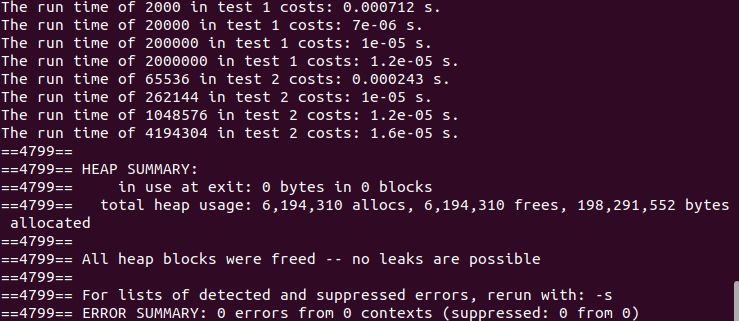
\includegraphics[scale = 0.5]{memory leak}

test 1:最差案例,test 2: 平均案列。从以上的测试结果可知,最差案例比平均案例的运行时间更慢。使用valgrind测试程序泄漏。显然,以上程序没有内存泄漏。


\end{document}
